\documentclass[crop,tikz]{standalone}
\usetikzlibrary{backgrounds}
\colorlet{blue}{cyan}
\tikzset{
  inverted/.style = {
    color=white,
    background rectangle/.style={fill},
    show background rectangle
  }
}

\usepackage{pgfplots}

\pgfplotsset{
  inverted/.style = {
    every axis legend/.append style={
      draw=white,
      fill=black,
      text=white
    }
  }
}

\tikzset{>=latex}
\colorlet{green}{green}

\begin{document}
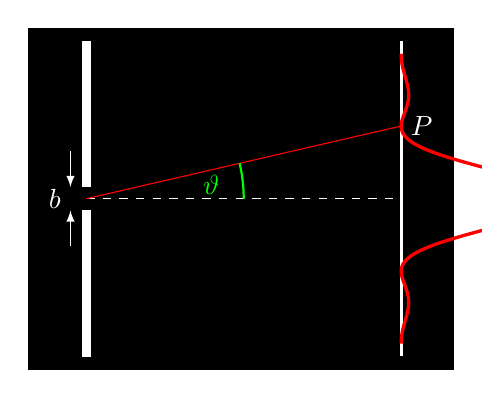
\begin{tikzpicture}[inverted,inverted]
  \pgfmathsetlengthmacro{\slitmax}{2cm}
  \pgfmathsetlengthmacro{\slitx}{0cm}
  \pgfmathsetlengthmacro{\slity}{0cm}
  \pgfmathsetlengthmacro{\slitheight}{0.3cm}
  \pgfmathsetlengthmacro{\slitwidth}{0.1cm}
  \pgfmathsetlengthmacro{\distance}{4cm}
  \pgfmathsetmacro{\angl}{13}
  \pgfmathsetlengthmacro{\boffset}{0.2cm}
  \pgfmathsetlengthmacro{\radius}{2cm}
  % slit
  \draw[fill] ({\slitx-\slitwidth/2},{\slity+\slitheight/2}) rectangle ({\slitwidth/2},{\slitmax});
  \draw[fill] ({\slitx-\slitwidth/2},{\slity-\slitheight/2}) rectangle ({\slitwidth/2},{-\slitmax});
  \draw[->] ({\slitx-\boffset},{\slity-2*\slitheight}) -- ++ (0,{ 3*\slitheight/2});
  \draw[->] ({\slitx-\boffset},{\slity+2*\slitheight}) -- ++ (0,{-3*\slitheight/2});
  \node[left] at ({\slitx-\boffset},{\slity}) {$b$};
  % ray
  \draw[dashed] ({\slitx},{\slity}) -- ++ ({\distance},0);
  \draw[red] ({\slitx},{\slity}) -- ({\angl}:{\distance/cos(\angl)}) coordinate (P);
  \draw[green,thick] (\radius,0) arc (0:\angl:\radius);
  \node[green] at ({\angl/2}:{0.8*\radius}) { $\vartheta$ };
  % projection
  \draw[very thick] ({\slitx + \distance},{-\slitmax}) -- ({\slitx + \distance},{\slitmax});
  \node[right] at (P) {$P$};
  % intensity
  \begin{axis}[inverted,
    width={3*\slitmax},
    height={2*\slitmax},
    anchor=origin,
    rotate around={-90:(current axis.origin)},
    domain={-2*pi}:{2*pi},
    samples=100,
    smooth,
    axis x line=none,
    axis y line=none,
    yshift={\distance},
    declare function = { S(\x) = sin(deg(\x))^2/\x^2; },
    ]
    \addplot[red,very thick,smooth] { S(x) };
  \end{axis}
\end{tikzpicture}
\end{document}
